%%%%%%%%%%%%%%%%%%%% report.tex %%%%%%%%%%%%%%%%%%%%%%%%%%%%%%%%%%%
%
% Contribution to Springer "Advances in Experimental Medicine and Biology"
% Formatted using the SVMult document class (contributed volume)
%
%%%%%%%%%%%%%%%% Springer %%%%%%%%%%%%%%%%%%%%%%%%%%%%%%%%%%

% RECOMMENDED %%%%%%%%%%%%%%%%%%%%%%%%%%%%%%%%%%%%%%%%%%%%%%%%%%%
\documentclass[graybox]{svmult}

% ---- Required packages (Springer SVMult recommended set) ----
% \usepackage{type1cm}  % only needed if CM fonts are not scalable on your system
\usepackage{makeidx}
\usepackage{graphicx}
\usepackage{multicol}
\usepackage[bottom]{footmisc}
\usepackage[numbers]{natbib}

% ---- Additional packages needed for this contribution ----
\usepackage{amsmath,amssymb}
\let\Bbbk\relax  % resolve conflict between amssymb and newtxmath

\usepackage{newtxtext}
\usepackage[varvw]{newtxmath}

\usepackage{booktabs}
\usepackage{hyperref}
\usepackage{algorithm}
\usepackage{algorithmic}

\makeindex

%%%%%%%%%%%%%%%%%%%%%%%%%%%%%%%%%%%%%%%%%%%%%%%%%%%%%%%%%%%%%%%%%%%%%%%%%%%%%%%%%%%%%%%%%

\begin{document}

\title*{Latent Diffusion Models for Brain MRI Anomaly Detection and Synthetic Image Generation}
% Use \titlerunning{Short Title} for an abbreviated version of
% your contribution title if the original one is too long
\titlerunning{Latent Diffusion Models for Brain MRI Anomaly Detection}

\author{Georgios Manthos}
% Use \authorrunning{Short Title} for an abbreviated version of
% your contribution title if the original one is too long
\institute{Georgios Manthos \at Department of Digital Systems, University of Piraeus, Greece \and Institute of Information Technology, National Center for Scientific Research Demokritos, Greece, \email{gmanthos2@gmail.com}}
%
\maketitle

\abstract*{We present a two-stage latent diffusion framework for unsupervised brain tumor detection and synthetic medical image generation. A Variational Autoencoder (VAE) compresses $256 \times 256$ grayscale brain MRI slices into a compact $32 \times 32 \times 4$ latent representation, where a Denoising Diffusion Probabilistic Model (DDPM) with a U-Net backbone learns the distribution of healthy brain anatomy. For anomaly detection, input images are partially noised and reconstructed via Denoising Diffusion Implicit Models (DDIM) sampling conditioned on the healthy class using Classifier-Free Guidance (CFG); pixel-wise reconstruction errors then localize pathological regions such as tumors. For data augmentation, the model generates synthetic brain MRIs by sampling from the learned healthy distribution. We conduct an extensive hyperparameter ablation study across 120 configurations, evaluating the effects of diffusion checkpoint maturity, noise injection level ($t_\text{start}$), and guidance scale on detection performance. Our best configuration achieves an image-level AUROC of 0.756 and a pixel-level AUROC of 0.894 for tumor localization. Synthetic image quality is assessed via Fr\'{e}chet Inception Distance (FID = 144.43), Structural Similarity Index (SSIM), and Learned Perceptual Image Patch Similarity (LPIPS). Additionally, we provide model explainability through self-attention map visualization and denoising trajectory analysis, and discuss ethical considerations for the clinical deployment of generative models in medical imaging.}

\abstract{We present a two-stage latent diffusion framework for unsupervised brain tumor detection and synthetic medical image generation. A Variational Autoencoder (VAE) compresses $256 \times 256$ grayscale brain MRI slices into a compact $32 \times 32 \times 4$ latent representation, where a Denoising Diffusion Probabilistic Model (DDPM) with a U-Net backbone learns the distribution of healthy brain anatomy. For anomaly detection, input images are partially noised and reconstructed via Denoising Diffusion Implicit Models (DDIM) sampling conditioned on the healthy class using Classifier-Free Guidance (CFG); pixel-wise reconstruction errors then localize pathological regions such as tumors. For data augmentation, the model generates synthetic brain MRIs by sampling from the learned healthy distribution. We conduct an extensive hyperparameter ablation study across 120 configurations, evaluating the effects of diffusion checkpoint maturity, noise injection level ($t_\text{start}$), and guidance scale on detection performance. Our best configuration achieves an image-level AUROC of 0.756 and a pixel-level AUROC of 0.894 for tumor localization. Synthetic image quality is assessed via Fr\'{e}chet Inception Distance (FID = 144.43), Structural Similarity Index (SSIM), and Learned Perceptual Image Patch Similarity (LPIPS). Additionally, we provide model explainability through self-attention map visualization and denoising trajectory analysis, and discuss ethical considerations for the clinical deployment of generative models in medical imaging.\newline\indent
\textbf{Keywords:} diffusion models, anomaly detection, brain MRI, latent diffusion, synthetic medical images, DDPM, variational autoencoder, ethical AI, explainability}

% ============================================================
% 1. INTRODUCTION
% ============================================================
\section{Introduction}
\label{sec:introduction}

Medical imaging plays a central role in the diagnosis and monitoring of neurological disorders, with Magnetic Resonance Imaging (MRI) serving as the primary modality for detecting structural brain abnormalities such as tumors, lesions, and atrophy~\cite{baur2021autoencoders}. Despite its diagnostic value, the clinical deployment of automated analysis systems faces persistent challenges: annotated medical datasets are scarce due to the cost and expertise required for labeling, class distributions are heavily imbalanced (pathological cases are far less common than healthy ones), and privacy regulations constrain data sharing across institutions~\cite{yi2019generative}.

Traditional supervised approaches to brain tumor detection require large collections of pixel-level annotations, which are expensive and time-consuming to acquire. Furthermore, discriminative classifiers trained on limited datasets often fail to generalize across imaging protocols, scanner manufacturers, and patient demographics. These limitations have motivated growing interest in \textit{unsupervised} anomaly detection methods, which learn a model of normality exclusively from healthy data and identify pathology as deviations from this learned distribution~\cite{baur2021autoencoders, schlegl2019f}.

Generative models have emerged as a promising paradigm for both anomaly detection and data augmentation in medical imaging. Generative Adversarial Networks (GANs)~\cite{goodfellow2014generative} were among the first deep generative architectures applied to medical image synthesis~\cite{yi2019generative}, but they suffer from well-documented training instabilities, mode collapse, and limited diversity. More recently, Denoising Diffusion Probabilistic Models (DDPMs)~\cite{ho2020denoising} have demonstrated superior sample quality and training stability compared to GANs, achieving state-of-the-art results in natural image synthesis~\cite{dhariwal2021diffusion}. Latent Diffusion Models (LDMs)~\cite{rombach2022high} extend this paradigm by operating the diffusion process in a compressed latent space, dramatically reducing computational requirements while preserving generation quality.

In the context of medical anomaly detection, diffusion-based methods reconstruct pathological inputs as their healthy counterparts, and the resulting reconstruction error serves as an anomaly signal~\cite{wyatt2022anoddpm, wolleb2022diffusion, sanchez2022healthy}. This approach is particularly attractive because it requires \textit{no anomaly labels during training}---the model learns only from healthy examples and can detect arbitrary pathologies at inference time.

In this work, we present a complete latent diffusion pipeline for brain MRI analysis that serves a dual purpose: (1)~anomaly detection via reconstruction-error-based tumor localization, and (2)~high-quality synthetic brain MRI generation for potential data augmentation. Our contributions are as follows:

\begin{enumerate}
  \item We design and implement a two-stage latent diffusion architecture combining a MONAI-based Variational Autoencoder (VAE) with a class-conditional U-Net DDPM, featuring Classifier-Free Guidance (CFG) and DDIM sampling for efficient inference.
  \item We conduct a systematic hyperparameter ablation study across 120 configurations---spanning 10~model checkpoints, 4~noise injection levels, and 3~guidance scales---to characterize the sensitivity of anomaly detection performance to each factor.
  \item We provide quantitative evaluation of both anomaly detection (image-level and pixel-level AUROC) and synthetic image quality (FID, SSIM, LPIPS, diversity).
  \item We incorporate explainability mechanisms through self-attention map visualization and denoising trajectory analysis, and discuss ethical considerations for clinical deployment.
\end{enumerate}


% ============================================================
% 2. RELATED WORK
% ============================================================
\section{Related Work}
\label{sec:related_work}

\subsection{Denoising Diffusion Models}

Denoising Diffusion Probabilistic Models (DDPMs)~\cite{ho2020denoising} define a forward Markov chain that progressively corrupts data with Gaussian noise over $T$ timesteps, and a learned reverse process that iteratively denoises samples. The training objective is a simplified noise prediction loss:
\begin{equation}
\mathcal{L} = \mathbb{E}_{t, \mathbf{x}_0, \boldsymbol{\epsilon}} \left[ \| \boldsymbol{\epsilon} - \boldsymbol{\epsilon}_\theta(\mathbf{x}_t, t) \|^2 \right],
\label{eq:ddpm_loss}
\end{equation}
where $\boldsymbol{\epsilon}_\theta$ is a neural network (typically a U-Net) trained to predict the noise $\boldsymbol{\epsilon}$ added at timestep $t$. Song et al.~\cite{song2021denoising} introduced DDIM, a non-Markovian generalization enabling deterministic sampling with significantly fewer steps (e.g., 50 instead of 1000). Latent Diffusion Models (LDMs)~\cite{rombach2022high} further improve efficiency by applying the diffusion process in a compressed latent space via a pretrained autoencoder. Classifier-Free Guidance (CFG)~\cite{ho2022classifier} enables conditional generation without a separate classifier; at inference, the guided prediction combines conditional and unconditional outputs:
\begin{equation}
\tilde{\boldsymbol{\epsilon}} = \boldsymbol{\epsilon}_\theta(\mathbf{x}_t, t, \varnothing) + w \cdot \left( \boldsymbol{\epsilon}_\theta(\mathbf{x}_t, t, c) - \boldsymbol{\epsilon}_\theta(\mathbf{x}_t, t, \varnothing) \right),
\label{eq:cfg}
\end{equation}
where $w$ is the guidance scale and $\varnothing$ denotes the null (unconditional) class token.

\subsection{Anomaly Detection in Medical Imaging}

Unsupervised anomaly detection in medical imaging follows a reconstruction-based paradigm: a generative model trained exclusively on healthy data identifies anomalies as regions with high reconstruction error~\cite{baur2021autoencoders}. Early VAE-based approaches~\cite{kingma2014auto} produced blurry reconstructions, while GAN-based methods such as f-AnoGAN~\cite{schlegl2019f} suffered from optimization instabilities. Diffusion-based anomaly detection has emerged as a compelling alternative: AnoDDPM~\cite{wyatt2022anoddpm} uses simplex noise and partial noising for brain MRI anomaly detection; Wolleb et al.~\cite{wolleb2022diffusion} condition the reverse process on a healthy class to ``correct'' pathological regions; Sanchez et al.~\cite{sanchez2022healthy} frame detection as counterfactual healthy generation; and Behrendt et al.~\cite{behrendt2024patched} introduced patched diffusion models for improved localization.

\subsection{Synthetic Medical Image Generation}

GANs have been widely applied for medical image synthesis~\cite{yi2019generative}, but training instability and mode collapse remain challenges. Diffusion models have shown particular promise: Pinaya et al.~\cite{pinaya2022brain} demonstrated high-quality brain image generation using latent diffusion with MONAI~\cite{pinaya2023generative}, and Dorjsembe et al.~\cite{dorjsembe2022three} extended DDPMs to 3D medical volumes.
% ============================================================
% 3. METHODOLOGY
% ============================================================
\section{Methodology}
\label{sec:methodology}

Our pipeline follows a two-stage latent diffusion architecture. Stage~1 employs a Variational Autoencoder (VAE) that compresses brain MRI images into a compact latent space. Stage~2 trains a class-conditional DDPM in this latent space to model the distribution of healthy brain anatomy. At inference time, the system supports two operational modes: anomaly detection via partial noising and healthy-conditioned reconstruction, and synthetic image generation via full DDIM sampling.

\subsection{Variational Autoencoder (Stage 1)}
\label{sec:vae}

The VAE is based on the \texttt{AutoencoderKL} architecture from the MONAI framework~\cite{monai2022, pinaya2023generative}. It maps grayscale brain MRI images from pixel space $\mathbb{R}^{1 \times 256 \times 256}$ to a latent space $\mathbb{R}^{4 \times 32 \times 32}$, achieving an $8\times$ spatial downsampling with 4~latent channels.

The encoder follows a hierarchical structure with channel progression $[64, 128, 256, 256]$, employing 2~residual blocks per resolution level and self-attention at the two lowest resolutions. The decoder mirrors this architecture symmetrically. The training objective combines three loss terms:
\begin{equation}
\mathcal{L}_{\text{VAE}} = \mathcal{L}_{\text{L1}} + 0.5 \cdot \mathcal{L}_{\text{LPIPS}} + 10^{-6} \cdot \mathcal{L}_{\text{KL}},
\label{eq:vae_loss}
\end{equation}
where $\mathcal{L}_{\text{L1}}$ is the pixel-wise reconstruction loss, $\mathcal{L}_{\text{LPIPS}}$ is the perceptual loss~\cite{zhang2018perceptual}, and $\mathcal{L}_{\text{KL}}$ is the KL divergence regularization. The low KL weight ($\beta = 10^{-6}$) prioritizes reconstruction fidelity. The VAE was trained for 150 epochs with effective batch size 32, using AdamW ($\text{lr} = 10^{-4}$) and mixed-precision training.

\subsection{Latent Space Normalization}
\label{sec:normalization}

A critical implementation detail concerns the statistical properties of the VAE latent space. We observed that raw VAE latents exhibited a per-channel mean of approximately 0.86 and standard deviation of approximately 7.2---far from the standard normal distribution $\mathcal{N}(0, 1)$ assumed by the DDPM noise schedule. Operating the diffusion process on unnormalized latents caused the model to produce pure noise during generation, as the signal-to-noise ratio at each timestep was fundamentally miscalibrated.

To resolve this, we precompute per-channel mean $\boldsymbol{\mu}$ and standard deviation $\boldsymbol{\sigma}$ statistics across the entire training set and apply z-score normalization:
\begin{equation}
\mathbf{z}_{\text{norm}} = \frac{\mathbf{z}_{\text{raw}} - \boldsymbol{\mu}}{\boldsymbol{\sigma}}, \qquad
\mathbf{z}_{\text{raw}} = \mathbf{z}_{\text{norm}} \cdot \boldsymbol{\sigma} + \boldsymbol{\mu}.
\label{eq:normalization}
\end{equation}
Normalization is applied before DDPM training and forward noising; denormalization is applied after DDIM sampling and before VAE decoding. This step proved essential for successful training and is stored as a persistent statistics file for reproducibility.

\subsection{Denoising Diffusion Probabilistic Model (Stage 2)}
\label{sec:ddpm}

The DDPM operates in the normalized latent space using a U-Net architecture~\cite{ronneberger2015u} adapted for noise prediction. The U-Net processes $32 \times 32 \times 4$ latent tensors through an encoder--decoder structure with skip connections.

\paragraph{Architecture.} The U-Net uses a base channel width of 128 with channel multipliers $[1, 2, 4, 4]$, resulting in feature maps of $[128, 256, 512, 512]$ channels across four resolution levels ($32 \rightarrow 16 \rightarrow 8 \rightarrow 4$). Each level contains 2~residual blocks with GroupNorm and SiLU activations. Multi-head self-attention~\cite{vaswani2017attention} with 4~heads is applied at resolutions $16 \times 16$ and $8 \times 8$. A middle block with residual--attention--residual structure processes the $4 \times 4$ bottleneck. Gradient checkpointing is enabled throughout to fit within 8~GB VRAM.

\paragraph{Conditioning.} Timestep conditioning uses sinusoidal positional embeddings projected through a two-layer MLP. Class conditioning is implemented via a learned embedding table with 3~entries: healthy (class 0), anomalous (class 1), and a null token ($\varnothing$) for unconditional generation. The time and class embeddings are summed and injected into each residual block via additive conditioning.

\paragraph{Noise Schedule.} We employ a linear noise schedule with $\beta_{\text{start}} = 10^{-4}$ and $\beta_{\text{end}} = 0.02$ over $T = 1000$ timesteps. All derived quantities ($\alpha_t$, $\bar{\alpha}_t$, posterior coefficients) are precomputed for efficient training and sampling.

\paragraph{Training.} The model is trained for 200,000 steps with batch size 32, using AdamW (learning rate $2 \times 10^{-4}$, weight decay $0.01$), gradient clipping at norm 1.0, and mixed-precision training. An Exponential Moving Average (EMA)~\cite{polyak1992acceleration} of the model weights with decay $0.9999$ is maintained throughout training, and EMA weights are used for all inference. The training loss (Equation~\ref{eq:ddpm_loss}) converged to approximately $0.025$--$0.035$.

\subsection{Classifier-Free Guidance}
\label{sec:cfg}

During training, class labels are randomly replaced with the null token $\varnothing$ with probability $p = 0.1$, enabling the model to learn both conditional and unconditional noise prediction. At inference, the guided prediction follows Equation~\ref{eq:cfg}, where the guidance scale $w$ controls the strength of class conditioning. Higher guidance scales produce reconstructions more strongly biased toward the conditioned class, at the potential cost of reduced diversity and increased artifacts.

\subsection{Anomaly Detection Pipeline}
\label{sec:anomaly_pipeline}

The anomaly detection process is formalized in Algorithm~\ref{alg:anomaly}. Given an input brain MRI $\mathbf{x}$, the pipeline: (1)~encodes it to the latent space via the VAE encoder, (2)~normalizes the latent representation, (3)~adds noise at a specified timestep $t_{\text{start}}$ via the forward diffusion process, (4)~reconstructs a healthy version $\hat{\mathbf{x}}$ by running DDIM sampling conditioned on the healthy class (class 0) with CFG, (5)~denormalizes and decodes back to pixel space, and (6)~computes the anomaly map as the absolute pixel-wise difference $|\mathbf{x} - \hat{\mathbf{x}}|$, smoothed with a Gaussian filter ($\sigma = 2.0$). The global anomaly score is the mean of the raw (unnormalized) L1 error map.

\begin{algorithm}[t]
\caption{Diffusion-Based Anomaly Detection}
\label{alg:anomaly}
\begin{algorithmic}[1]
\REQUIRE Input image $\mathbf{x}$, noise level $t_{\text{start}}$, guidance scale $w$, DDIM steps $S$
\ENSURE Anomaly map $\mathbf{A}$, anomaly score $s$
\STATE $\mathbf{z}_0 \leftarrow \text{VAE}_{\text{enc}}(\mathbf{x})$ \COMMENT{Encode to latent space}
\STATE $\mathbf{z}_0^{\text{norm}} \leftarrow (\mathbf{z}_0 - \boldsymbol{\mu}) / \boldsymbol{\sigma}$ \COMMENT{Normalize}
\STATE $\boldsymbol{\epsilon} \sim \mathcal{N}(\mathbf{0}, \mathbf{I})$
\STATE $\mathbf{z}_{t} \leftarrow \sqrt{\bar{\alpha}_{t}} \, \mathbf{z}_0^{\text{norm}} + \sqrt{1 - \bar{\alpha}_{t}} \, \boldsymbol{\epsilon}$ \COMMENT{Forward noise}
\STATE $\hat{\mathbf{z}}_0^{\text{norm}} \leftarrow \text{DDIM}(\mathbf{z}_{t},\, c{=}\text{healthy},\, w,\, S)$ \COMMENT{Healthy reconstruction}
\STATE $\hat{\mathbf{z}}_0 \leftarrow \hat{\mathbf{z}}_0^{\text{norm}} \cdot \boldsymbol{\sigma} + \boldsymbol{\mu}$ \COMMENT{Denormalize}
\STATE $\hat{\mathbf{x}} \leftarrow \text{VAE}_{\text{dec}}(\hat{\mathbf{z}}_0)$ \COMMENT{Decode to pixel space}
\STATE $\mathbf{A}_{\text{raw}} \leftarrow |\mathbf{x} - \hat{\mathbf{x}}|$
\STATE $\mathbf{A} \leftarrow \text{GaussianSmooth}(\mathbf{A}_{\text{raw}}, \sigma{=}2.0)$
\STATE $s \leftarrow \text{mean}(\mathbf{A}_{\text{raw}})$ \COMMENT{Global anomaly score}
\RETURN $\mathbf{A}, s$
\end{algorithmic}
\end{algorithm}

The parameter $t_{\text{start}}$ controls the trade-off between anomaly destruction and anatomy preservation: higher values inject more noise (destroying more of the original signal, including both pathology and healthy structure), while lower values preserve more of the original anatomy but may fail to remove the anomaly. This trade-off is analyzed in detail in Section~\ref{sec:results}.

\subsection{Synthetic Image Generation}
\label{sec:generation}

For synthetic image generation, the pipeline performs full DDIM sampling starting from pure Gaussian noise $\mathbf{z}_T \sim \mathcal{N}(\mathbf{0}, \mathbf{I})$, conditioned on the healthy class with 50 deterministic DDIM steps ($\eta = 0$). The resulting normalized latent is denormalized and decoded through the VAE decoder to produce a $256 \times 256$ grayscale brain MRI.
% ============================================================
% 4. EXPERIMENTAL SETUP
% ============================================================
\section{Experimental Setup}
\label{sec:experiments}

\subsection{Dataset}
\label{sec:dataset}

We use the Brain Tumor Detection dataset~\cite{bhuvaji2020brain}, a publicly available collection of 2D brain MRI slices from Kaggle. The dataset comprises approximately 1,500 healthy and 1,500 anomalous (tumor-bearing) JPEG images of varying original dimensions. Ground truth tumor annotations are provided as VIA polygon masks in JSON format for a subset of anomalous images.

All images are preprocessed to $256 \times 256$ grayscale PNG format and normalized to the range $[-1, 1]$. The dataset is split into training (70\%), validation (15\%), and test (15\%) partitions. The test set contains 225 healthy and 450 anomalous images. Importantly, the DDPM is trained \textit{exclusively} on healthy images (via their precomputed latent representations), following the unsupervised anomaly detection paradigm.

\subsection{Implementation Details}
\label{sec:implementation}

The pipeline is implemented in PyTorch 2.12 with MONAI~\cite{monai2022} for the VAE. All experiments run on a single NVIDIA RTX 4060 (8~GB VRAM), using gradient checkpointing, automatic mixed precision, and consolidated latent storage ($\sim$17~MB single tensor file) to fit within memory constraints. Table~\ref{tab:hyperparameters} summarizes the key hyperparameters.

\begin{table}[!t]
\caption{Training hyperparameters for the two-stage pipeline}
\label{tab:hyperparameters}
\begin{tabular}{p{3.5cm}p{3.5cm}p{3.5cm}}
\hline\noalign{\smallskip}
\textbf{Parameter} & \textbf{VAE (Stage 1)} & \textbf{DDPM (Stage 2)} \\
\noalign{\smallskip}\svhline\noalign{\smallskip}
Input resolution    & $256 \times 256 \times 1$ & $32 \times 32 \times 4$ \\
Channels            & $[64, 128, 256, 256]$ & $[128, 256, 512, 512]$ \\
Residual blocks     & 2 per level & 2 per level \\
Attention           & Levels 3--4 & Res.\ $16 \times 16$, $8 \times 8$ \\
Optimizer           & AdamW & AdamW \\
Learning rate       & $1 \times 10^{-4}$ & $2 \times 10^{-4}$ \\
Weight decay        & 0.01 & 0.01 \\
Batch size          & 4 (eff.\ 32) & 32 \\
Training duration   & 150 epochs & 200K steps \\
EMA decay           & 0.999 & 0.9999 \\
Gradient clipping   & 1.0 & 1.0 \\
Mixed precision     & Yes & Yes \\
\noalign{\smallskip}\hline\noalign{\smallskip}
\end{tabular}
\end{table}

\subsection{Evaluation Metrics}
\label{sec:metrics}

\paragraph{Anomaly Detection.} We evaluate anomaly detection at two levels:
\begin{itemize}
  \item \textbf{Image-level}: Each image receives a scalar anomaly score (mean raw L1 reconstruction error). We report the Area Under the Receiver Operating Characteristic curve (AUROC), Area Under the Precision--Recall Curve (AUPRC), F1-score at the optimal threshold, sensitivity (true positive rate), and specificity (true negative rate).
  \item \textbf{Pixel-level}: Using ground truth polygon masks, we compute pixel-level AUROC by treating each pixel's anomaly map value as a prediction and the binary mask as ground truth.
\end{itemize}

\paragraph{Synthetic Image Quality.} We assess generation quality using FID~\cite{heusel2017gans} (distributional distance), SSIM~\cite{wang2004image} (structural similarity), LPIPS~\cite{zhang2018perceptual} (perceptual distance), and intra-set diversity (LPIPS between generated pairs). SSIM and LPIPS are computed over 200 randomly sampled cross-distribution pairs.
% ============================================================
% 5. RESULTS
% ============================================================
\section{Results}
\label{sec:results}

\subsection{Anomaly Detection Performance}
\label{sec:anomaly_results}

Table~\ref{tab:anomaly_results} presents the anomaly detection performance for the best configuration identified through our grid search: checkpoint \texttt{step\_100000}, $t_{\text{start}} = 150$, and guidance scale $w = 7.5$. This configuration achieves an image-level AUROC of 0.756 and AUPRC of 0.851, demonstrating meaningful discrimination between healthy and anomalous brain MRIs using only unsupervised training on healthy data.

\begin{table}[!t]
\caption{Image-level anomaly detection performance (best configuration)}
\label{tab:anomaly_results}
\begin{tabular}{p{3cm}p{3cm}}
\hline\noalign{\smallskip}
\textbf{Metric} & \textbf{Value} \\
\noalign{\smallskip}\svhline\noalign{\smallskip}
AUROC        & 0.756 \\
AUPRC        & 0.851 \\
F1-Score     & 0.784 \\
Sensitivity  & 0.784 \\
Specificity  & 0.564 \\
Precision    & 0.783 \\
\noalign{\smallskip}\hline\noalign{\smallskip}
\end{tabular}
\end{table}

At the pixel level, using ground truth polygon tumor masks, our model achieves a pixel-level AUROC of \textbf{0.894}, indicating strong localization capability. Figure~\ref{fig:roc_curve} shows the pixel-level ROC curve, and Figure~\ref{fig:qualitative} presents a qualitative example comparing the original MRI, ground truth tumor mask, and the generated anomaly heatmap.

\begin{figure}[t]
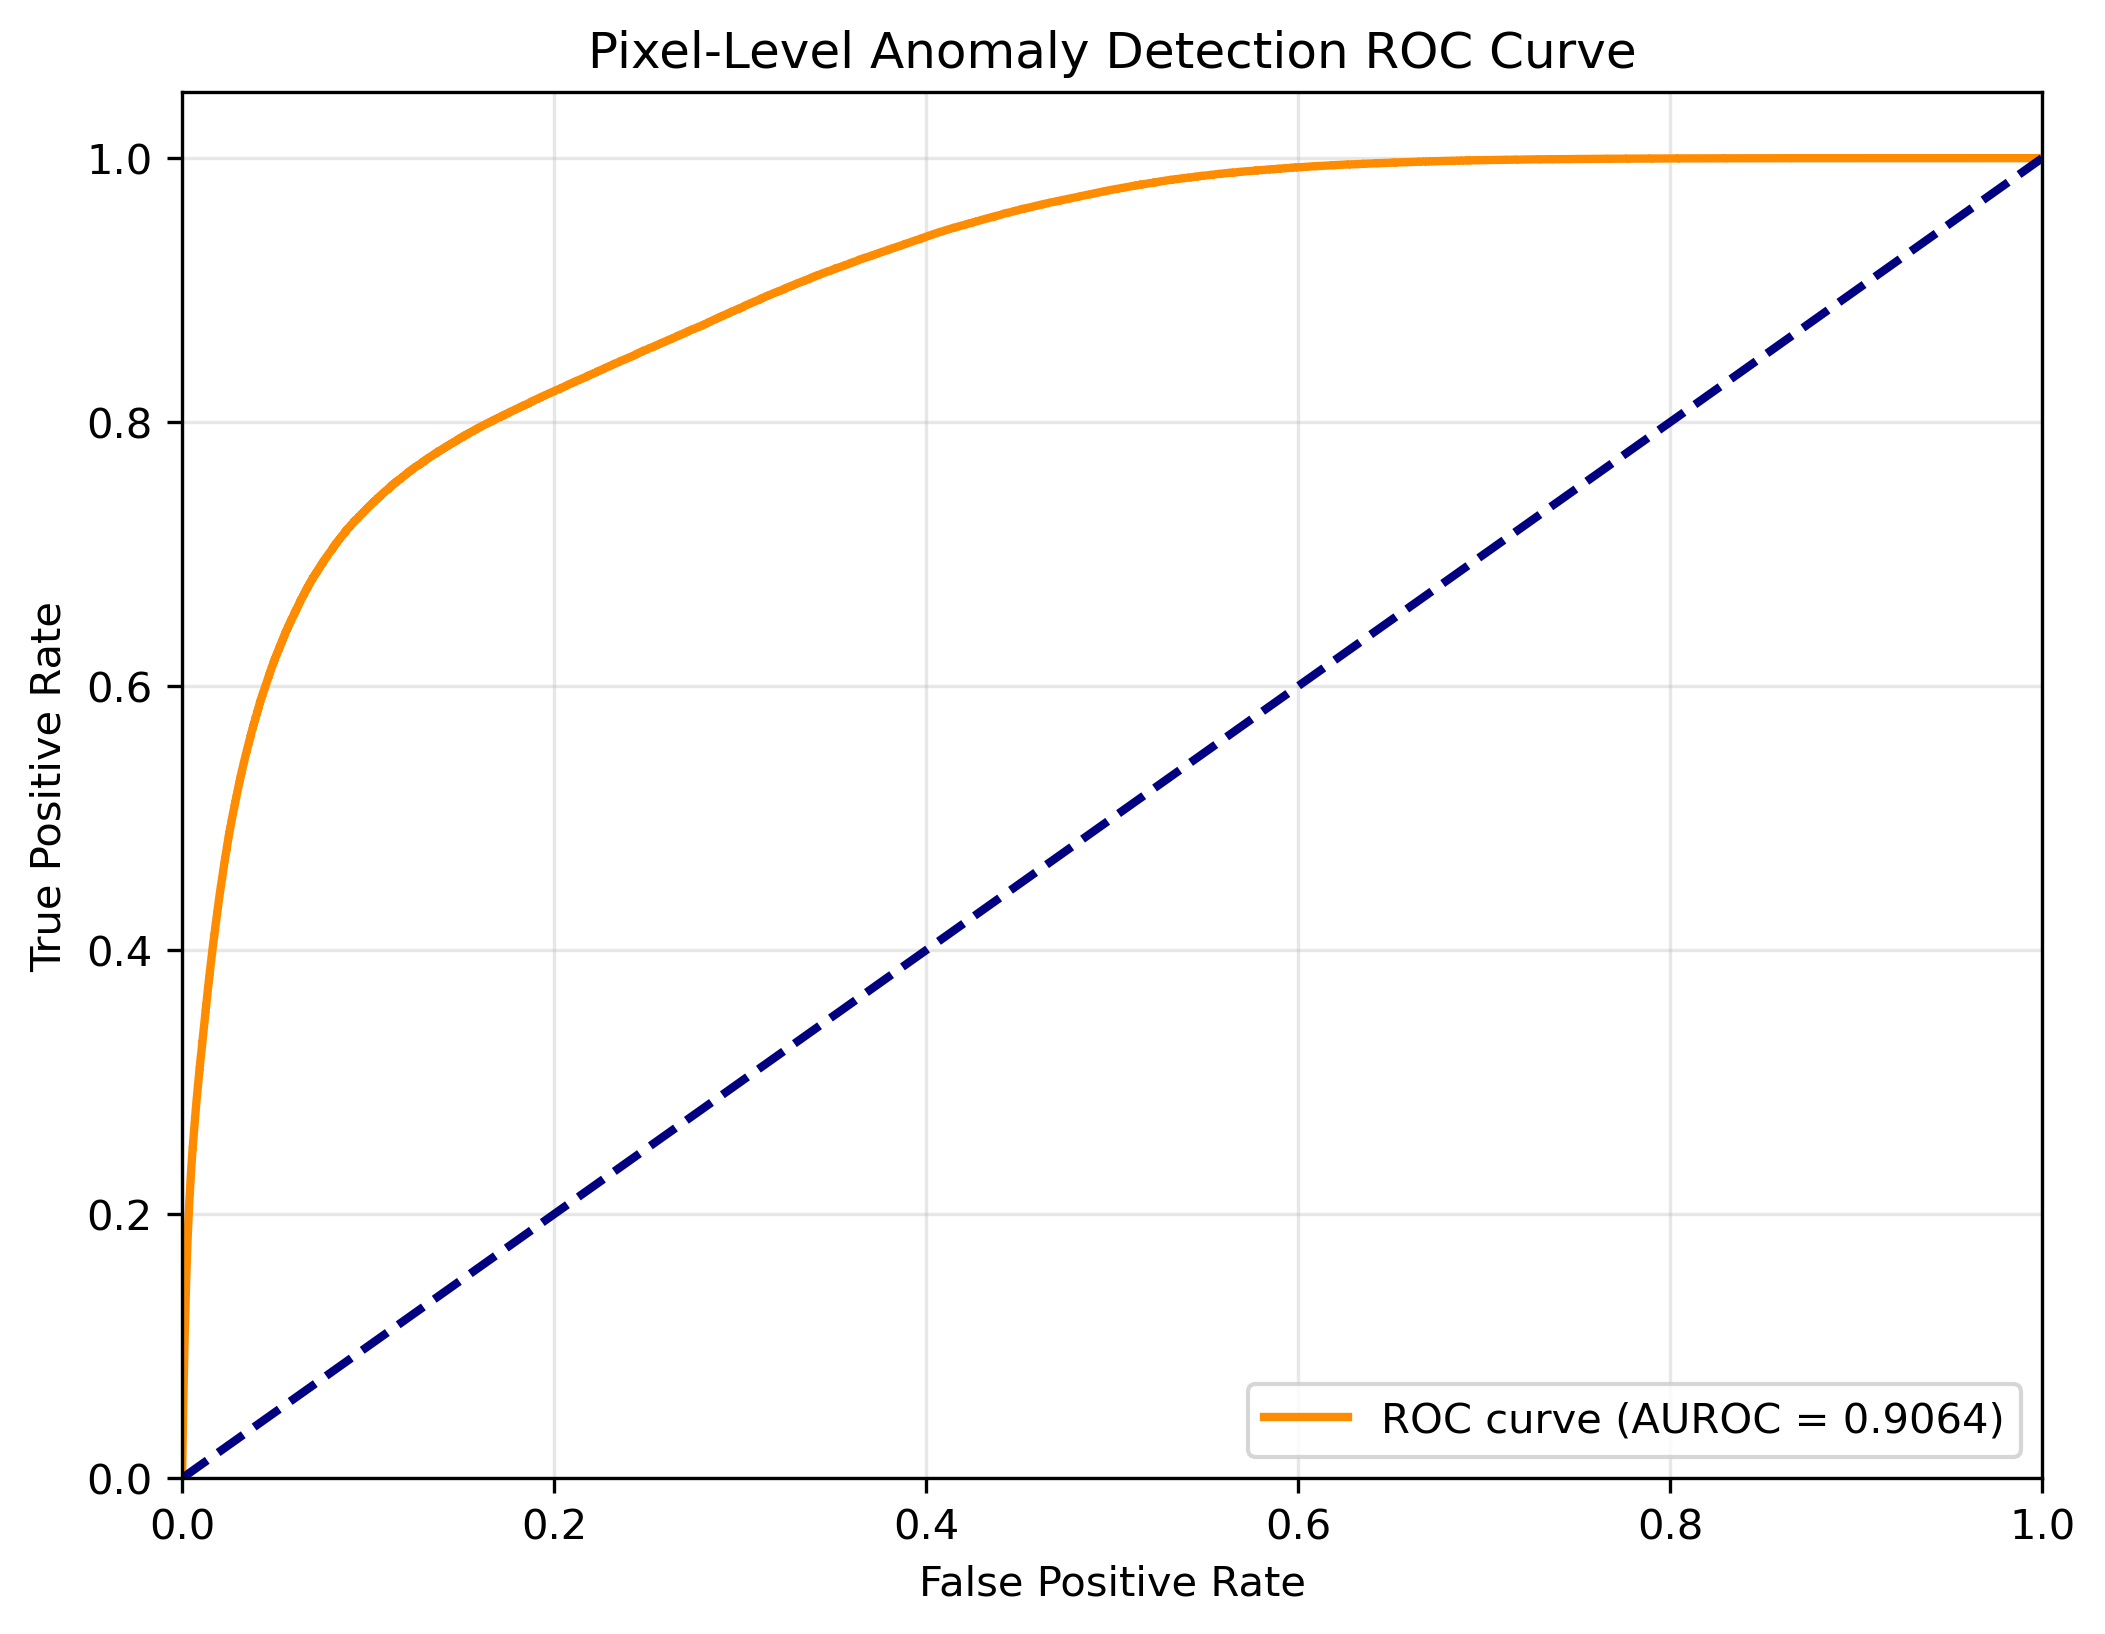
\includegraphics[width=0.65\textwidth]{../results/evaluation/roc_curve_pixel_level.png}
\caption{Pixel-level ROC curve for anomaly localization (AUROC = 0.894). The model demonstrates strong ability to discriminate tumor pixels from healthy tissue based on reconstruction error}
\label{fig:roc_curve}
\end{figure}

\begin{figure}[t]
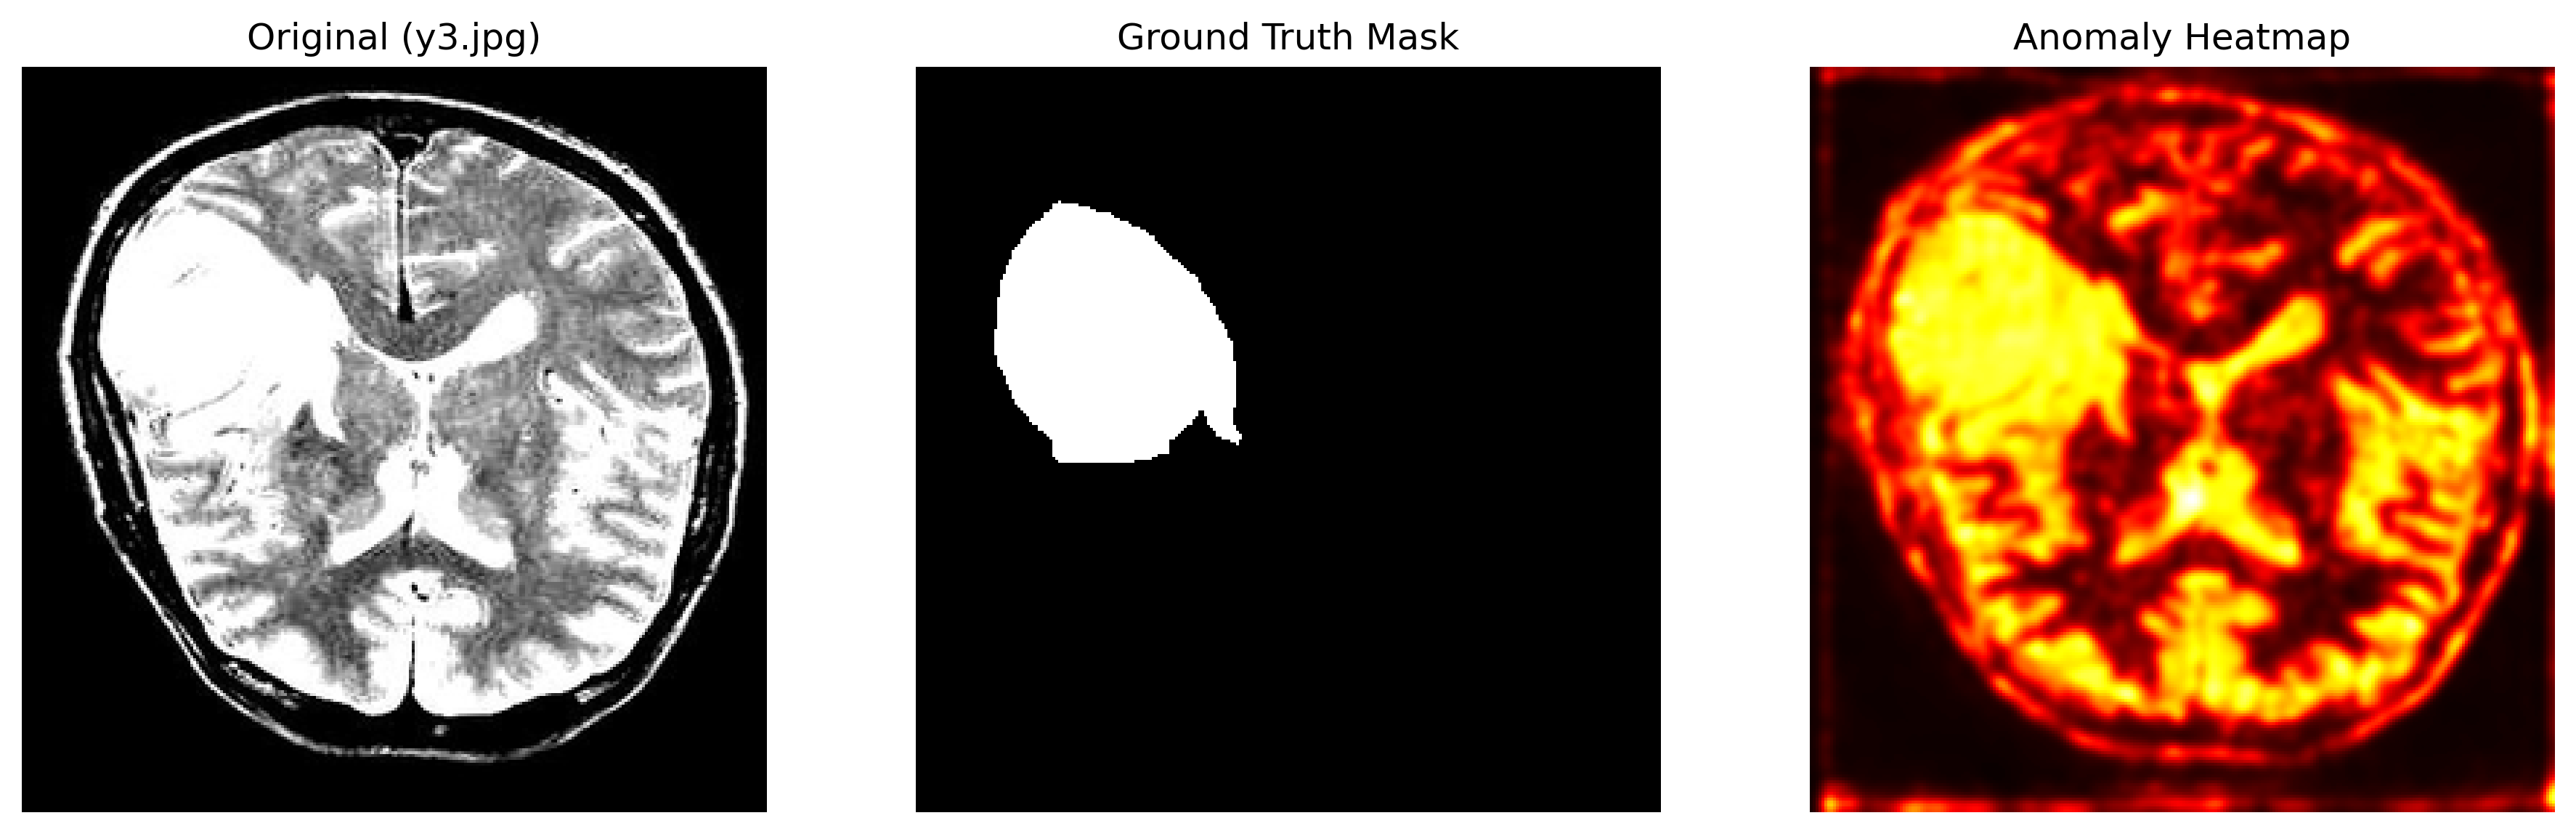
\includegraphics[width=\textwidth]{../results/evaluation/qualitative_example_1.png}
\caption{Qualitative anomaly detection example. Left to right: original brain MRI with tumor, ground truth tumor mask, healthy reconstruction, and anomaly heatmap generated by our diffusion-based reconstruction pipeline. High-intensity regions in the heatmap correspond to areas where the healthy reconstruction deviates from the original, successfully localizing the tumor}
\label{fig:qualitative}
\end{figure}

We also note that lowering the guidance scale to $w = 3.0$ (same checkpoint and $t_{\text{start}}$) yields a high-sensitivity configuration with sensitivity of \textbf{0.880} and F1 of 0.820, at the cost of reduced specificity (0.467). This trade-off is clinically relevant: a screening tool may prioritize sensitivity to avoid missing tumors, while a diagnostic tool may require balanced precision and recall.

\subsection{Hyperparameter Ablation Study}
\label{sec:grid_search}

We conducted an extensive grid search across 120 configurations: 10 training checkpoints (50K--140K steps, in 10K increments) $\times$ 4 noise injection levels ($t_{\text{start}} \in \{150, 200, 250, 300\}$) $\times$ 3 guidance scales ($w \in \{3.0, 5.0, 7.5\}$). Table~\ref{tab:top_configs} presents the top 5 configurations ranked by AUROC.

\begin{table}[!t]
\caption{Top 5 hyperparameter configurations by image-level AUROC (grid search over 120 combinations)}
\label{tab:top_configs}
\begin{tabular}{p{1.8cm}p{1cm}p{0.8cm}p{1.2cm}p{0.8cm}p{1cm}p{1cm}}
\hline\noalign{\smallskip}
\textbf{Checkpoint} & $\boldsymbol{t_{\textbf{start}}}$ & $\boldsymbol{w}$ & \textbf{AUROC} & \textbf{F1} & \textbf{Sens.} & \textbf{Spec.} \\
\noalign{\smallskip}\svhline\noalign{\smallskip}
step\_100K & 150 & 7.5 & \textbf{0.756} & 0.784 & 0.784 & 0.564 \\
step\_80K  & 200 & 7.5 & 0.755 & 0.754 & 0.711 & 0.649 \\
step\_100K & 150 & 3.0 & 0.755 & \textbf{0.820} & \textbf{0.880} & 0.467 \\
step\_140K & 150 & 3.0 & 0.755 & 0.785 & 0.784 & 0.573 \\
step\_100K & 150 & 5.0 & 0.755 & 0.742 & 0.689 & 0.662 \\
\noalign{\smallskip}\hline\noalign{\smallskip}
\end{tabular}
\end{table}

\paragraph{Effect of Noise Injection Level ($t_{\text{start}}$).} The noise injection level emerges as the most critical hyperparameter. Table~\ref{tab:tstart_effect} shows performance at different $t_{\text{start}}$ values with the best checkpoint (step\_100K) and guidance scale ($w = 7.5$) held fixed. At $t_{\text{start}} = 150$, AUROC is maximized at 0.756. Higher values progressively degrade performance: at $t_{\text{start}} = 250$, AUROC drops to 0.739, and at $t_{\text{start}} = 400$, it falls to approximately 0.649. This confirms that excessive noising destroys healthy anatomical features along with pathology, while insufficient noising fails to remove the anomaly signal.

\begin{table}[!t]
\caption{Effect of noise injection level $t_{\text{start}}$ on anomaly detection (step\_100K, $w = 7.5$)}
\label{tab:tstart_effect}
\begin{tabular}{p{1.5cm}p{1.5cm}p{1.5cm}p{2cm}p{2cm}}
\hline\noalign{\smallskip}
$\boldsymbol{t_{\textbf{start}}}$ & \textbf{AUROC} & \textbf{F1} & \textbf{Sensitivity} & \textbf{Specificity} \\
\noalign{\smallskip}\svhline\noalign{\smallskip}
150  & \textbf{0.756} & 0.784 & 0.784 & 0.564 \\
200  & 0.749 & 0.767 & 0.738 & 0.627 \\
250  & 0.739 & 0.793 & 0.811 & 0.529 \\
400  & 0.649 & 0.539 & 0.402 & 0.818 \\
\noalign{\smallskip}\hline\noalign{\smallskip}
\end{tabular}
\end{table}

\paragraph{Effect of Guidance Scale ($w$).} The guidance scale exhibits a more nuanced effect: while AUROC remains relatively stable across guidance values (varying by less than 0.002), the guidance scale modulates the sensitivity--specificity trade-off. At $w = 3.0$, the model achieves the highest sensitivity (0.880) but lowest specificity (0.467); at $w = 7.5$, the balance shifts toward higher specificity (0.564) with moderate sensitivity (0.784). This behavior suggests that stronger guidance produces more conservative healthy reconstructions, reducing false positives at the cost of some false negatives.

\paragraph{Effect of Checkpoint Maturity.} The checkpoint at 100K training steps consistently produces the best AUROC across different hyperparameter combinations. Earlier checkpoints (50K--90K) show marginally lower AUROC, indicating incomplete convergence. Later checkpoints (110K--140K) show comparable but slightly reduced performance, suggesting mild overfitting to training data patterns.

\subsection{Synthetic Image Quality}
\label{sec:generation_results}

Table~\ref{tab:generation_metrics} presents the quantitative evaluation of 500 synthetic brain MRI images generated using checkpoint step\_100K with DDIM sampling (50 steps, $\eta = 0$, conditioned on healthy class).

\begin{table}[!t]
\caption{Synthetic image generation quality metrics (500 generated images vs.\ real healthy test images)}
\label{tab:generation_metrics}
\begin{tabular}{p{5cm}p{4cm}}
\hline\noalign{\smallskip}
\textbf{Metric} & \textbf{Value} \\
\noalign{\smallskip}\svhline\noalign{\smallskip}
FID $\downarrow$                      & 144.43 \\
SSIM $\uparrow$                       & $0.129 \pm 0.085$ \\
LPIPS $\downarrow$                    & $0.534 \pm 0.033$ \\
Diversity (LPIPS) $\uparrow$          & $0.404 \pm 0.104$ \\
\noalign{\smallskip}\hline\noalign{\smallskip}
\end{tabular}
\end{table}

The FID of 144.43 reflects moderate generation quality, contextualized by our small training set ($\sim$1,500 images) and the limited calibration of ImageNet-based FID for grayscale medical imagery. The intra-set diversity (LPIPS = 0.404) confirms varied sample generation without mode collapse.

\subsection{Explainability Analysis}
\label{sec:explainability_results}

To enhance interpretability, we provide two complementary explainability mechanisms. Figure~\ref{fig:attention_maps} visualizes self-attention weights from the U-Net's attention layers at resolutions $16 \times 16$ and $8 \times 8$ during denoising. The attention maps reveal that the model focuses on anatomically meaningful structures---ventricular boundaries, cortical folds, and tissue interfaces---providing evidence of learned brain anatomy representations. Figure~\ref{fig:denoising_trajectory} compares the denoising trajectory for a healthy and an anomalous brain MRI. For healthy inputs, reconstruction converges smoothly to the original; for anomalous inputs, the model progressively ``corrects'' the tumor region, replacing it with healthy-appearing tissue---the mechanism underlying our anomaly detection.

\begin{figure}[t]
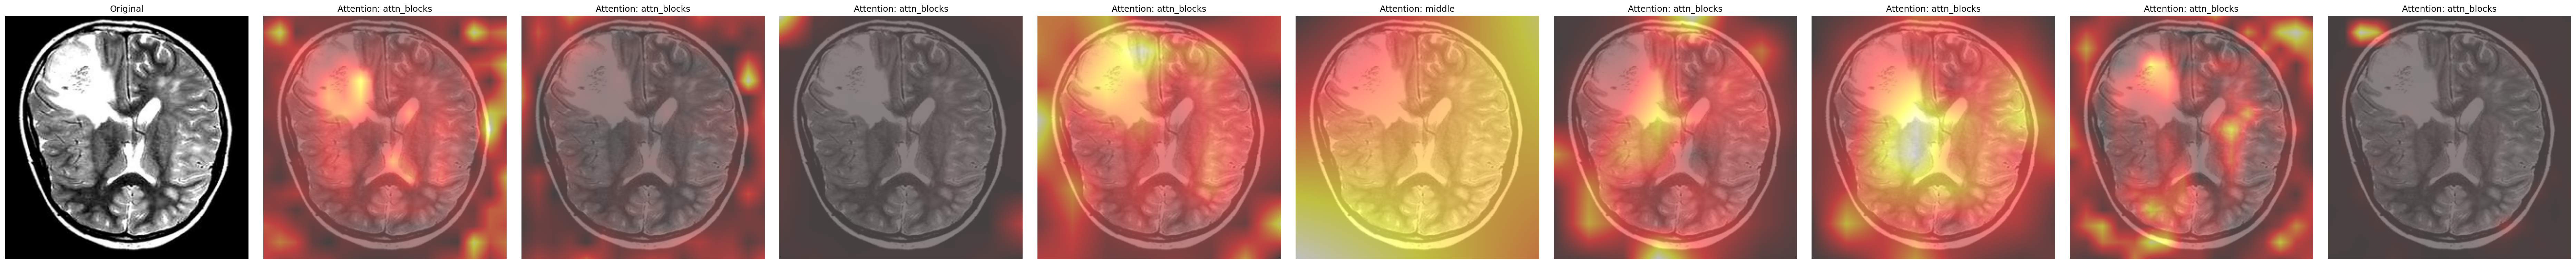
\includegraphics[width=\textwidth]{../results/explainability/attention_maps.png}
\caption{Self-attention maps from the U-Net during denoising. The model attends to anatomically relevant structures, demonstrating learned spatial awareness of brain morphology}
\label{fig:attention_maps}
\end{figure}

\begin{figure}[t]
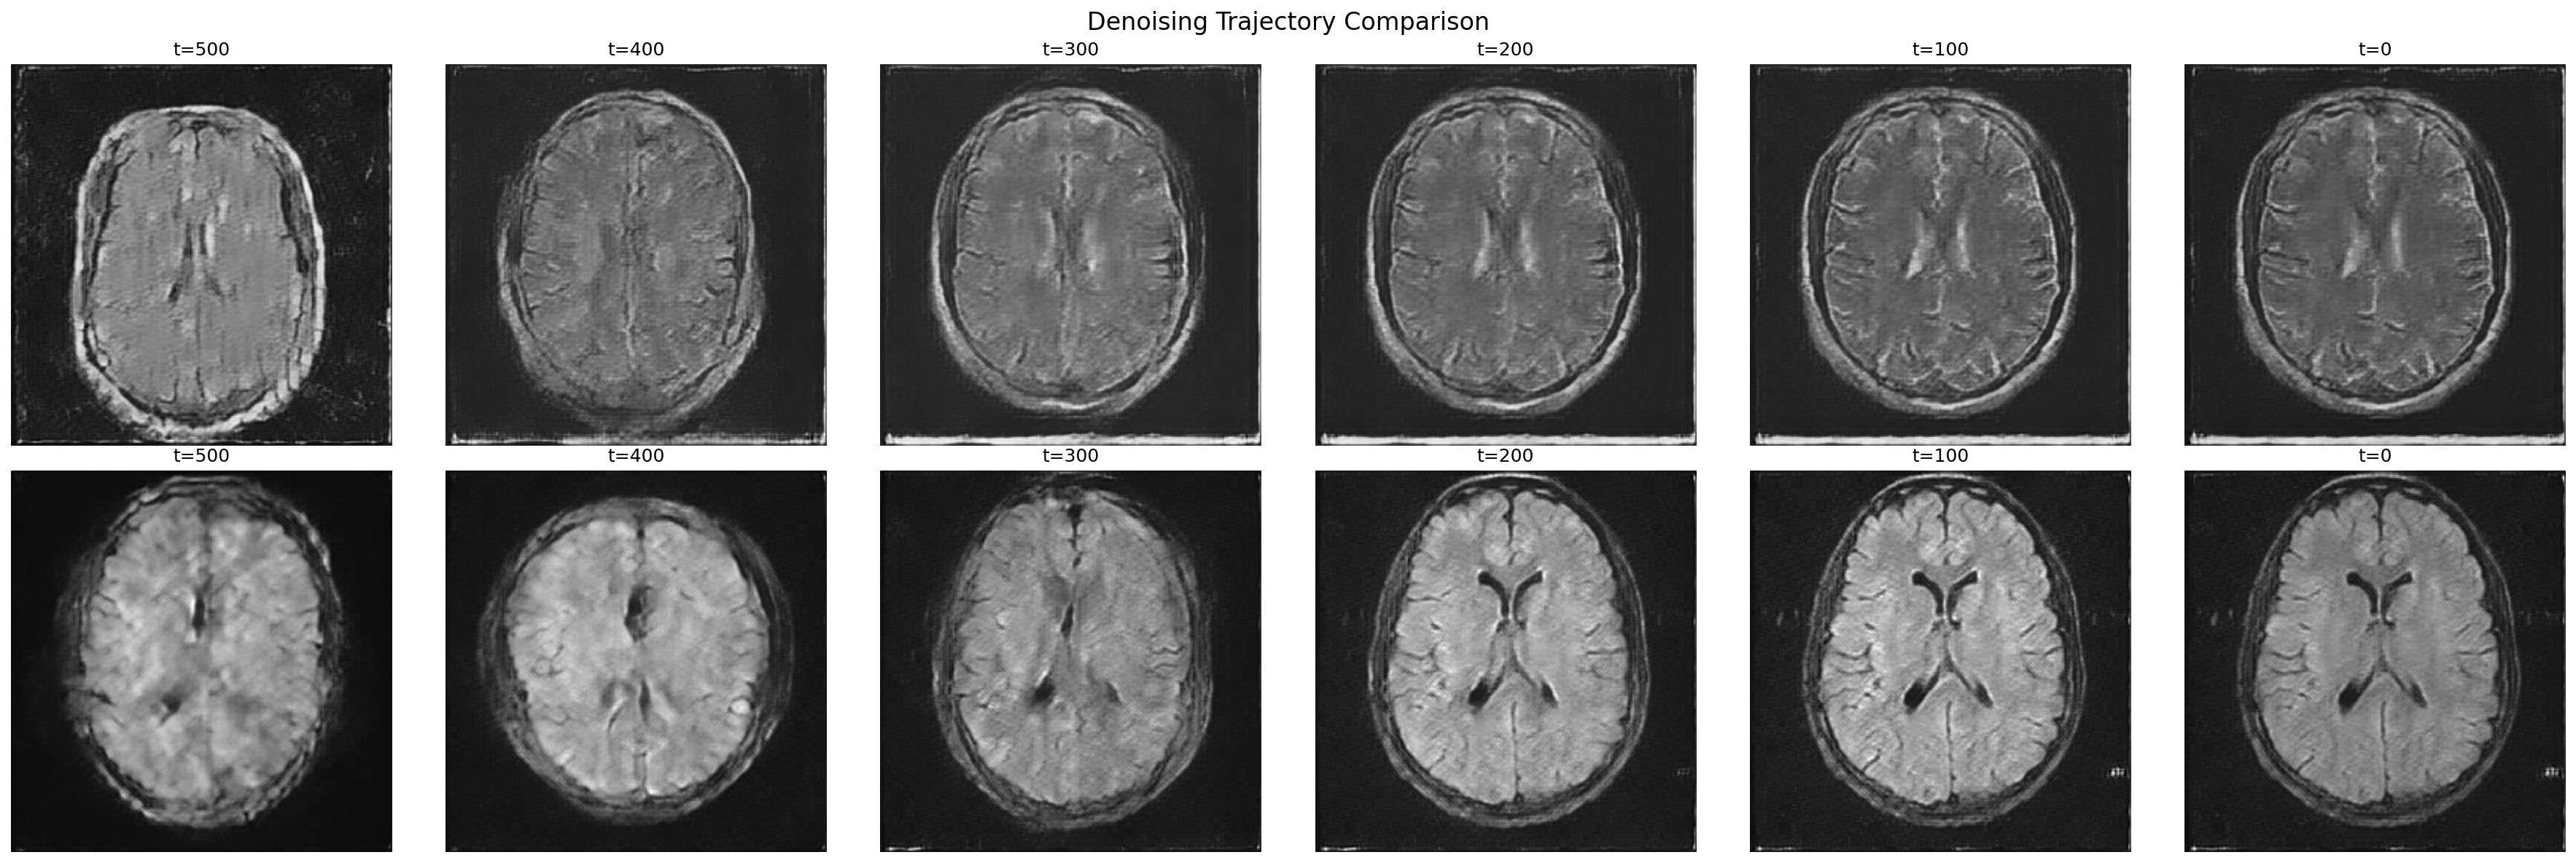
\includegraphics[width=\textwidth]{../results/explainability/denoising_trajectory_comparison.png}
\caption{Denoising trajectory comparison between a healthy brain MRI (top) and a tumor-bearing MRI (bottom). The healthy-conditioned reconstruction progressively ``corrects'' the tumor region}
\label{fig:denoising_trajectory}
\end{figure}
% ============================================================
% 6. DISCUSSION
% ============================================================
\section{Discussion}
\label{sec:discussion}

\paragraph{Anomaly Detection Mechanism.} Our results demonstrate that latent diffusion models can effectively detect brain tumors through reconstruction-based anomaly scoring, without requiring any anomaly labels during training. The core mechanism relies on the model's inability to faithfully reconstruct pathological regions when conditioned on the healthy class: since the DDPM has only learned the distribution of healthy brain anatomy, it ``corrects'' anomalous regions during healthy-conditioned reconstruction, producing measurable reconstruction error in tumor areas.

\paragraph{Critical Role of $t_{\text{start}}$.} The hyperparameter ablation study reveals that the noise injection level $t_{\text{start}}$ is the most influential factor in anomaly detection performance. This parameter controls a fundamental trade-off: sufficient noise must be injected to destroy the anomaly signal in the latent representation, but excessive noise also destroys healthy anatomical features, causing the model to hallucinate new anatomy during reconstruction and generating false positive errors. Our optimal value of $t_{\text{start}} = 150$ (out of $T = 1000$) corresponds to a moderate noise level that balances these competing objectives. This finding aligns with observations in AnoDDPM~\cite{wyatt2022anoddpm} and other reconstruction-based methods.

\paragraph{Guidance Scale as a Clinical Tuning Knob.} The guidance scale $w$ provides a clinically useful sensitivity--specificity trade-off with minimal impact on overall AUROC. At $w = 3.0$, the model achieves 88\% sensitivity (detecting the vast majority of tumors) at the cost of more false positives. At $w = 7.5$, the model is more conservative, with balanced sensitivity and specificity. This tunable behavior could be valuable in clinical deployment, where the cost asymmetry between missed tumors and false alarms varies across applications (screening vs.\ diagnostic confirmation).

\paragraph{Generation Quality Context.} The FID of 144.43, while moderate compared to natural image benchmarks, should be interpreted in context. Our model is trained on approximately 1,500 single-channel grayscale images---a small dataset by generative modeling standards. The FID metric itself is calibrated for RGB natural images and may not accurately capture medical image quality. The intra-set diversity score (LPIPS = 0.404) confirms meaningful sample variety, and qualitative inspection shows anatomically plausible brain MRI generations.

\paragraph{Comparison with Related Methods.} Direct comparison with existing methods is challenging due to differences in datasets, preprocessing, and evaluation protocols. However, our image-level AUROC of 0.756 falls within the range reported by comparable methods: AnoDDPM~\cite{wyatt2022anoddpm} achieves AUROCs of 0.70--0.83 depending on the anomaly type and noise configuration, while Wolleb et al.~\cite{wolleb2022diffusion} report 0.74--0.86 on brain tumor datasets. Our pixel-level AUROC of 0.894 is competitive, demonstrating strong localization despite operating at a coarse latent resolution ($32 \times 32$) that is upsampled to $256 \times 256$ by the VAE decoder.

\paragraph{Inference Efficiency.} With CFG and $S = 50$ DDIM steps, each anomaly detection pass requires $2S = 100$ U-Net forward evaluations. Operating in the $32 \times 32$ latent space rather than $256 \times 256$ pixel space reduces per-pass FLOPs by $\sim$$50\times$, and DDIM's $20\times$ step reduction over full DDPM sampling yields an overall $\sim$$1000\times$ speedup versus a na\"{i}ve pixel-space baseline. In practice, inference completes in $\sim$300--350~ms per image ($\sim$3~images/s) on an NVIDIA RTX 4060, with a total model footprint of $\sim$52M parameters (35M U-Net + 17M VAE).

\paragraph{Limitations.} Several limitations should be acknowledged:
\begin{itemize}
  \item \textbf{2D processing}: Our model operates on individual 2D slices, ignoring volumetric context that could improve detection of spatially coherent pathologies.
  \item \textbf{Limited dataset}: The Brain Tumor Detection dataset contains approximately 3,000 images from a single source, limiting the diversity of brain anatomy and imaging conditions represented.
  \item \textbf{No demographic metadata}: The dataset provides no patient demographics, precluding analysis of potential performance disparities across populations.
  \item \textbf{Resolution bottleneck}: The $8\times$ spatial compression by the VAE limits the finest anomaly localization resolution to approximately $8 \times 8$ pixel patches in the original image space.
  \item \textbf{No clinical validation}: All evaluations are performed on benchmark data; clinical deployment would require prospective validation with radiologist assessment.
\end{itemize}

\paragraph{Ethical and Regulatory Considerations.} Deploying generative AI in medical imaging raises important concerns. \textit{Data privacy}: diffusion models trained on small datasets risk memorizing individual examples~\cite{akbar2023beware, dar2024investigating}; mitigations include perceptual similarity monitoring and differential privacy. \textit{Dataset bias}: the absence of demographic metadata precludes fairness analysis, and non-representative training data may cause normal anatomical variants to be flagged as anomalies. \textit{Synthetic data safety}: generated images must not substitute for real diagnostic data and should carry ``SYNTHETIC'' provenance labels. Any clinical application would require compliance with the EU AI Act and FDA SaMD guidance, including prospective validation, IRB approval, and regulatory clearance. This work is a research prototype and is \textbf{not suitable for clinical diagnosis}.

% ============================================================
% 7. CONCLUSION
% ============================================================
\section{Conclusion}
\label{sec:conclusion}

We have presented a two-stage latent diffusion pipeline for brain MRI anomaly detection and synthetic image generation. The system combines a MONAI-based VAE for perceptual compression with a class-conditional U-Net DDPM operating in the normalized latent space, using DDIM sampling and Classifier-Free Guidance for efficient inference.

Our systematic evaluation demonstrates that the pipeline achieves an image-level AUROC of 0.756 and a pixel-level AUROC of 0.894 for tumor localization, competitive with existing diffusion-based anomaly detection methods. A comprehensive hyperparameter ablation study across 120 configurations reveals that the noise injection level $t_{\text{start}}$ is the dominant factor in detection performance, while the guidance scale provides a clinically useful sensitivity--specificity trade-off. The model also generates diverse synthetic brain MRIs with an FID of 144.43.

We further contribute explainability mechanisms and discuss ethical considerations for responsible clinical deployment. Future work includes 3D volumetric processing, larger multi-institutional datasets, multi-modal conditioning, and prospective clinical validation.

% ============================================================
% ACKNOWLEDGMENTS
% ============================================================
\begin{acknowledgement}
The authors acknowledge the creators of the Brain Tumor Detection dataset on Kaggle for making their data publicly available, and the MONAI Consortium for their open-source medical imaging framework. All computations were performed on a consumer-grade NVIDIA RTX 4060 GPU, demonstrating the accessibility of latent diffusion methods for medical imaging research.
\end{acknowledgement}

% ============================================================
% BIBLIOGRAPHY
% ============================================================
\bibliographystyle{spbasic}
\bibliography{references}

\end{document}
